\chapter{Arquitetura Proposta}
\label{cap:arquitetura}

Este capítulo descreve a arquitetura de \textit{backend} concebida para suprir as lacunas consolidadas na Seção \ref{sec:resultados-msl}. A exposição parte dos requisitos e da lacuna que origina cada um, registra as decisões estruturantes, descreve as camadas lógicas, a modelagem semântica das entidades e os componentes que constituem a contribuição deste trabalho, e encerra com um cenário de missão crítica.

\section{Visão Geral e Princípios de Projeto}
\label{sec:visao-geral}

A arquitetura organiza-se em cinco camadas lógicas em torno de um núcleo semântico único, seguindo um modelo de referência de gêmeos digitais urbanos em cinco camadas. A Figura \ref{fig:arquitetura} apresenta a organização resultante, com os macro componentes e as interfaces de dados entre eles, isto é, o que cada componente consome e fornece. As setas rotulam essas interfaces e não a sequência de um caso de uso particular, que varia conforme o cenário e aparece na Seção \ref{sec:cenario}.

\begin{figure}[!htbp]
    \centering

    \begin{minipage}{0.80\textwidth}
        
        \caption{Macrocomponentes da arquitetura proposta, por camada}
        \label{fig:arquitetura}
        \centering
        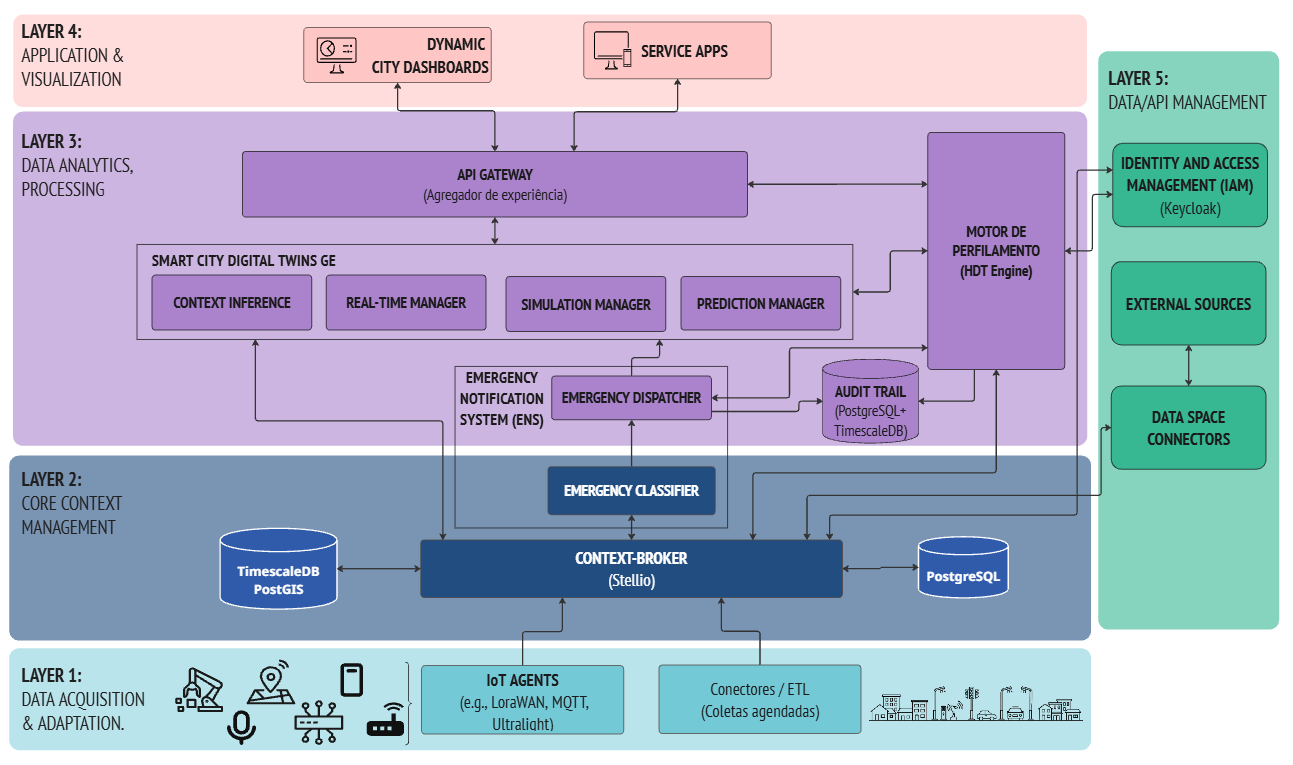
\includegraphics[width=\linewidth]{Imagens/fig_arquitetura.png}

        \par
        \raggedright
        \footnotesize
        \legend{Fonte: elaborada pelo autor sobre o modelo de referência em cinco camadas.}
    \end{minipage}
\end{figure}

Cinco princípios derivados das lacunas do mapeamento governam o desenho: fonte única de verdade, integração assíncrona, separação entre representação e política, persistência especializada e componente trocável fora do contêiner que o usa. O contexto urbano tem fonte única de verdade, de modo que infraestrutura, evento e pessoa são entidades NGSI-LD no \textit{Context Broker} e nenhum serviço mantém representação paralela desse estado. A integração entre o núcleo e os componentes de aplicação é assíncrona e declarativa. A representação está separada da política, com o modelo semântico descrevendo o que existe e os componentes de domínio o que fazer. A persistência é especializada por perfil de acesso. Por fim, componente que se pretenda trocável fica externo ao contêiner que o utiliza, critério que explica por que o Motor de Perfilamento e o \textit{Emergency Notification System} não residem dentro do bloco de processamento de contexto.

\section{Requisitos e Rastreabilidade}
\label{sec:requisitos}

A Tabela \ref{tab:requisitos} enuncia os requisitos funcionais (RF) e não funcionais (RNF), cada um com indicação da lacuna que o motiva. Com essa rastreabilidade, a avaliação do Capítulo \ref{cap:avaliacao} verifica atendimento de requisito, em vez de aferir desempenho de forma genérica.

O limiar de RNF1, de 1~s no percentil 95 e 2~s no percentil 99 (Tabela \ref{tab:requisitos}), é uma meta de projeto, e não um valor normativo: nenhuma norma encontrada define a latência de um \textit{backend} de notificação personalizada. A referência mais próxima é o prazo de 4~s que a 3GPP TS 22.268 fixa para a entrega ao terminal da notificação primária de alerta de terremoto e tsunami, que não inclui o \textit{backend} \cite{etsi2026ts122268}. Atribui-se ao \textit{backend} metade desse prazo, de modo que a cadeia completa fique em até 6~s no pior caso. Sistemas de alerta urbano medem, em trechos distintos do de RNF1, de dezenas a centenas de milissegundos \cite{maltezos2022smart,zhang2025developing}, o que deixa margem para a travessia de grafo e as regras.

\begin{table}[H]
\centering
\caption{Requisitos funcionais e não funcionais, com a lacuna de origem}
\label{tab:requisitos}
\scriptsize
\begin{tabularx}{\textwidth}{@{}l X l@{}}
\toprule
\textbf{Código} & \textbf{Requisito} & \textbf{Lacuna} \\
\midrule
RF1 & Ingerir dados de contexto em conformidade com NGSI-LD, validando o \texttt{@context} declarado e rejeitando \textit{payloads} semanticamente inconsistentes. & L1, L3 \\
RF2 & Representar o perfil do cidadão como entidade NGSI-LD de primeira classe, com relacionamentos navegáveis para entidades de infraestrutura e de evento. & L1 \\
RF3 & Registrar toda mudança de estado de contexto em um \textit{log} durável e ordenado, recuperável para reprocessamento. & L2 \\
RF4 & Admitir o registro de assinaturas declarativas que disparem notificação quando critérios de atributo, geografia ou relacionamento sejam satisfeitos, com endereço de notificação declarado pelo próprio assinante. & L2, L3 \\
RF5 & Derivar, a partir de um evento crítico, os destinatários da resposta, afetados e atuantes, por travessia de grafo combinada a predicado geoespacial e a critério de atributo. & L1, L3 \\
RF6 & Avaliar regras de personalização sobre o conjunto derivado e emitir resposta diferenciada por perfil, incluindo rota de evacuação compatível com as restrições declaradas e instrução de atuação a quem tem competência verificada. & L3 \\
RF7 & Consolidar telemetria de uso e atributos declarados em atualizações incrementais da entidade de perfil, com registro de proveniência por atributo. & L1 \\
RF8 & Materializar o estado corrente georreferenciado e o histórico de atributos em mecanismos de persistência distintos. & L5 \\
RF9 & Condicionar o acesso a atributos de perfil à autorização do núcleo semântico integrada ao serviço de identidade, registrando em trilha de auditoria a finalidade declarada e a decisão tomada. & L4 \\
RF10 & Expor aos clientes contratos agregados por caso de uso, com o recorte de contexto personalizado por pessoa, ocultando a topologia interna de serviços. & L2 \\
\midrule
RNF1 & Latência fim-a-fim entre a ingestão do evento crítico e a emissão da notificação personalizada, em até 1~s no percentil 95 e em até 2~s no percentil 99. & L2, L3 \\
RNF2 & Durabilidade das mensagens de contexto, sem perda de eventos críticos sob pico de carga. & L2 \\
RNF3 & Escalabilidade horizontal independente por serviço, sem reimplantação do núcleo semântico. & L2 \\
RNF4 & Tolerância à indisponibilidade de consumidores não críticos, sem interrupção da ingestão. & L2 \\
RNF5 & Minimização dos dados pessoais processados, restringindo a propagação de atributos sensíveis ao estritamente necessário à decisão. & L4 \\
RNF6 & Explicabilidade da decisão de personalização, com registro da regra aplicada e dos atributos considerados. & L4 \\
RNF7 & Reprodutibilidade integral do ambiente por infraestrutura declarada como código. & L5 \\
RNF8 & Extensibilidade do modelo semântico a novos domínios sem alteração dos serviços existentes. & L1 \\
\bottomrule
\end{tabularx}
\legend{Fonte: elaborada pelo autor.}
\end{table}

\section{Decisões Arquiteturais}
\label{sec:adr}

As sete decisões estruturantes, designadas DA1 a DA7, seguem uma ordem de dependência, e cada uma delimita o espaço de escolha da seguinte. São registradas segundo a prática de registro de decisão arquitetural recomendada por \citeonline{bass2021software}: o problema que resolvem, as alternativas consideradas, a escolha e a consequência aceita. Quando a justificativa é raciocínio de projeto, e não evidência, o texto o declara. DA1, DA2 e DA7 são detalhadas em texto, e DA3 a DA6 constam das Tabelas \ref{tab:adr} e \ref{tab:adr2}.

\subsection{Modelo de informação e interface de contexto (DA1)}

O modelo de informação precisa dar três coisas ao fluxo que leva um evento urbano à pessoa afetada: relacionamentos entre cidadão, edificação e evento que se possam percorrer (RF5), assinatura de mudanças por atributo, geografia ou relacionamento (RF4) e um vocabulário que um domínio novo estenda sem alterar os serviços existentes (RNF8). Esses requisitos vêm das lacunas L1 a L3 (Seção \ref{sec:resultados-msl}).

Três alternativas foram consideradas: o NGSI-v2, o NGSI-LD e uma API REST própria por domínio. O NGSI-v2 liga entidades só por convenção de nome (Seção \ref{sec:contexto}), e por isso a travessia (RF5) e a extensão do vocabulário (RNF8) ficam a cargo de cada aplicação. A API própria teria de construir as assinaturas (RF4) e exigiria alterar os serviços existentes a cada domínio novo (RNF8). O NGSI-LD atende aos três na mesma interface: trata relacionamentos como parte do modelo, especifica as assinaturas e declara o vocabulário no \texttt{@context}, que um domínio novo estende sem alterar os demais \cite{etsi2024ngsild}.

Portanto, depois dessa análise, o NGSI-LD foi adotado. Como o JSON-LD é uma serialização do RDF, o NGSI-LD mantém a base semântica do grafo sem exigir banco RDF nem SPARQL \cite{fiware2026catalogue,abid2022toward}. O custo é a complexidade: é preciso entender JSON-LD \cite{fiware2026tutorials}, e a interface fica presa à versão da especificação, hoje a TS 104 175 da ETSI \cite{etsi2026ts104175}.

\subsection{Implementação do \textit{Context Broker} (DA2)}

Adotado o NGSI-LD, resta escolher quem o implementa. O pré-requisito é oferecer os recursos de DA1, e quatro critérios da Seção \ref{sec:requisitos} comparam as candidatas: o registro durável das mudanças (RF3, RNF2), a escalabilidade por serviço (RNF3, estendida por raciocínio de projeto aos serviços internos do broker), a autenticação e a autorização nativas (RF9) e a latência fim a fim (RNF1), da qual o broker responde por uma parcela. Um quinto critério é de projeto: a coerência da persistência com DA4.

O catálogo do FIWARE lista três implementações com NGSI-LD \cite{fiware2026catalogue}, comparadas na Tabela \ref{tab:brokers} a partir da documentação de cada projeto e de duas avaliações de desempenho \cite{ntallaris2024benchmarking,lazidis2022publish}.

\begin{table}[!tp]
\centering
\caption{Implementações NGSI-LD de \textit{Context Broker} consideradas}
\label{tab:brokers}
\scriptsize
\begin{tabularx}{\textwidth}{@{}>{\raggedright\arraybackslash}p{2.5cm}>{\raggedright\arraybackslash}X>{\raggedright\arraybackslash}X>{\raggedright\arraybackslash}X@{}}
\toprule
\textbf{Atributo} & \textbf{Orion-LD} & \textbf{Scorpio} & \textbf{Stellio} \\
\midrule
Arquitetura & Processo único, em C/C++. & Microsserviços em Java, sobre \textit{Spring Cloud} e, em versão recente, \textit{Quarkus}. & Microsserviços em Kotlin, sobre \textit{Spring Boot} e \textit{Spring Cloud}. \\
\addlinespace
Cobertura da API NGSI-LD & Subconjunto dos \textit{endpoints}, segundo o catálogo; conformidade quase total com a versão 1.6.1, segundo o projeto. & Interface temporal opcional. & Interfaces de núcleo, temporal e de assinatura, em serviços distintos. \\
\addlinespace
Barramento interno & Sem barramento entre serviços; consumidor Kafka opcional para ingestão. & Kafka entre os serviços. & Kafka entre os serviços, com um evento por operação, publicado após o \textit{commit}. \\
\addlinespace
Persistência & MongoDB; histórico opcional em PostgreSQL com PostGIS e TimescaleDB. & PostgreSQL com PostGIS, inclusive nas consultas temporais \cite{ntallaris2024benchmarking}. & PostgreSQL com as extensões Timescale e PostGIS. \\
\addlinespace
Autenticação e autorização & Sem OAuth2 nativo \cite{lazidis2022publish}. & OAuth2 para autenticação e autorização \cite{lazidis2022publish,scorpio2026docs}; modelo de permissão não detalhado. & Nativas e opcionais, por OpenID Connect e OAuth2, validadas com Keycloak; permissão por entidade, tipo e escopo. \\
\addlinespace
\textit{Context Sources} e operação distribuída & Registro de \textit{Context Sources} e operações distribuídas, segundo o projeto. & Implantação centralizada, distribuída ou federada; fontes de contexto podem ser outros brokers. & Registro de \textit{Context Sources} e recuperação de entidades relacionadas nelas; operação distribuída em desenvolvimento. \\
\bottomrule
\end{tabularx}
\legend{Fonte: elaborada pelo autor, a partir de \cite{fiware2026catalogue,fiware2026orionld,scorpio2026docs,stellio2025docs}.}
\end{table}

O Orion-LD sai da comparação por três motivos: o registro durável, a escalabilidade e a persistência. O processo único não tem barramento entre serviços, e a tolerância a falhas exige um escalonador e um \textit{cluster} de brokers e de MongoDB \cite{ntallaris2024benchmarking}; por raciocínio de projeto, o \textit{log} de RF3 teria de ser montado fora do broker, e a escala só viria por réplica do processo inteiro. No Stellio, o serviço de busca publica cada evento no Kafka depois do \textit{commit} e na ordem do \textit{commit} \cite{stellio2025docs}. Sob carga alta, as arquiteturas em microsserviços escalam melhor que o Orion-LD \cite{ntallaris2024benchmarking}. Na persistência, o Orion-LD guarda o estado corrente em MongoDB e o histórico em PostgreSQL, dois motores de famílias distintas, enquanto DA4 fixa PostgreSQL com PostGIS e TimescaleDB. O critério de latência favorece o Orion-LD, mas prevalecem o registro durável e a escalabilidade, porque, por raciocínio de projeto, um alerta perdido custa mais do que centenas de milissegundos.

Entre Scorpio e Stellio, o pré-requisito e a escalabilidade não separam as candidatas: ambas são microsserviços ligados por Kafka, guardam o estado corrente em PostgreSQL com PostGIS e respondem de forma semelhante sob carga crescente \cite{ntallaris2024benchmarking,lazidis2022publish}, e \citeonline{lazidis2022publish} consideram o Scorpio o mais completo em funcionalidade. A decisão repousa em duas razões de alinhamento, a persistência e a identidade, e em uma razão prática, nenhuma medida neste trabalho. Na persistência, o Stellio guarda o histórico em TimescaleDB e o estado corrente em PostGIS, a combinação de DA4, enquanto no Scorpio todas as consultas do \textit{benchmark} rodaram em PostGIS; nesse \textit{benchmark}, o Stellio foi mais robusto na consulta temporal mais custosa, indício indireto, e não prova \cite{ntallaris2024benchmarking}. Na identidade, os dois usam OAuth2 \cite{lazidis2022publish}, mas só o Stellio documenta permissões por entidade, tipo e escopo, validadas com Keycloak \cite{stellio2025docs}. A razão prática, a familiaridade do autor com o Spring, pesa menos, porque o Spring também está na base de uma versão do Scorpio. O Stellio registra \textit{Context Sources} \cite{stellio2025docs}, recurso de que DA5 depende, e o encaminhamento das demais operações será testado na versão instalada.

Adota-se o Stellio \cite{stellio2025docs} com a opção \texttt{fail}. As consequências aceitas são cinco: o custo de implantação, a rejeição de escritas com o Kafka indisponível, o risco de latência, a reversibilidade parcial e a ausência de suporte a NGSI-v1 e NGSI-v2 \cite{fiware2026catalogue}. A pilha mínima inclui o barramento interno e um PostgreSQL com dois bancos. A opção \texttt{fail} troca disponibilidade da ingestão por consistência do registro: com uma única réplica do Kafka, como na prova de conceito, a indisponibilidade detectada vira escrita rejeitada, e a saída para produção é replicar o barramento, e não relaxar a opção. O risco de latência vem das avaliações, em que o Orion-LD ingeriu mais rápido por lote \cite{ntallaris2024benchmarking} e respondeu mais rápido em publicação e assinatura \cite{lazidis2022publish}, e a decisão deve ser revista se a latência medida no Capítulo \ref{cap:avaliacao} não couber em RNF1. A reversibilidade é parcial: trocar de broker altera a implantação, a integração com o Keycloak e o modelo de permissões de DA7, mas não os consumidores NGSI-LD, salvo diferenças de versão e cobertura. O Motor de Perfilamento e o \textit{Emergency Notification System} não leem o Kafka e se acoplam ao broker só pela assinatura NGSI-LD, embora dependam dele indiretamente, porque é por ele que o serviço de assinaturas recebe as mudanças que disparam as notificações \cite{stellio2025docs}.

\subsection{Integração, persistência, contexto derivado e regras (DA3 a DA6)}

A Tabela \ref{tab:adr} reúne DA3 e DA4, e a Tabela \ref{tab:adr2}, DA5 e DA6.

\begin{table}[H]
\centering
\caption{Decisões arquiteturais sobre a integração por assinatura e a persistência}
\label{tab:adr}
\scriptsize
\begin{tabularx}{\textwidth}{@{}l>{\raggedright\arraybackslash}p{3.1cm}XX@{}}
\toprule
\textbf{Código} & \textbf{Problema e decisão} & \textbf{Alternativas descartadas} & \textbf{Consequência aceita} \\
\midrule
DA3 & Definir como os componentes de domínio tomam conhecimento das mudanças de contexto (RNF2, RNF4). Adota-se a assinatura NGSI-LD como integrador primário, com endereço de notificação declarado por cada assinante. & Consumo direto do barramento interno do broker, que exigiria montar o evento no formato interno da implementação e criaria acoplamento de versão; consulta periódica ao broker, incompatível com RNF1. & Consistência eventual entre o núcleo e as visões derivadas, exigindo que as consultas tolerem defasagem limitada. \\
\addlinespace
DA4 & Atender consulta geoespacial sobre estado corrente e agregação sobre série histórica, de requisitos de indexação incompatíveis (RF8, RNF3). Adota-se a persistência que o próprio núcleo opera, PostgreSQL com PostGIS \cite{obe2021postgis} e TimescaleDB \cite{timescale2025docs}, escolha corroborada empiricamente \cite{john2023application,rudakov2023comparison,simanjuntak2022multiple}. A trilha de auditoria de RF9 usa uma instância própria do mesmo motor (DA7). & Persistência unificada de propósito geral, pela degradação previsível de um dos perfis; banco de séries temporais isolado, pela ausência de predicados geométricos; réplica do contexto em bases próprias dos componentes, por contrariar a fonte única de verdade; banco de documentos para a trilha, por introduzir um terceiro paradigma de persistência no capítulo em que a persistência excluiu um concorrente (DA2). & Os componentes de domínio passam a depender do desempenho de consulta do núcleo, que se torna objeto de medição no Capítulo \ref{cap:avaliacao}, e as consultas temporais custam caro em todos os brokers avaliados \cite{ntallaris2024benchmarking}. \\
\bottomrule
\end{tabularx}
\legend{Fonte: elaborada pelo autor.}
\end{table}

\begin{table}[H]
\centering
\caption{Decisões arquiteturais sobre o contexto derivado e a derivação da resposta}
\label{tab:adr2}
\scriptsize
\begin{tabularx}{\textwidth}{@{}l>{\raggedright\arraybackslash}p{3.1cm}XX@{}}
\toprule
\textbf{Código} & \textbf{Problema e decisão} & \textbf{Alternativas descartadas} & \textbf{Consequência aceita} \\
\midrule
DA5 & Entregar o contexto derivado pelos gestores sem expor a topologia interna do bloco. Registra-se o bloco no broker como \textit{Context Source} NGSI-LD \cite{etsi2024ngsild}. & Expor o bloco só por ligações diretas, sem registro no broker, o que multiplicaria interfaces e deixaria o contexto derivado invisível a quem consulta apenas o broker. & A consulta encaminhada é síncrona, logo gestor cujo cálculo não cabe no tempo da requisição precisa pré-computar e publicar o resultado como entidade. \\
\addlinespace
DA6 & Derivar a resposta personalizada de forma auditável (RNF6). Adota-se, nesta etapa, motor de regras determinístico e explicável sobre o grafo semântico, exigência derivada da lacuna L4 e dos riscos de discriminação por perfil inferido \cite{fontes2024human}. & Modelo estatístico opaco, que não permitiria registrar a regra aplicada e os atributos considerados em cada decisão; arranjos híbridos \cite{lex2025hybrid} ficam como evolução posterior, sem ruptura arquitetural. & Menor capacidade de generalização para padrões não antecipados na especificação das regras. \\
\bottomrule
\end{tabularx}
\legend{Fonte: elaborada pelo autor.}
\end{table}

A consequência de DA3 merece uma explicação além da tabela. Pela assinatura, o núcleo avisa cada assinante quando um dado muda, sem que um componente precise conhecer os outros \cite{eugster2003many}. O aviso chega um instante depois da mudança, e nesse intervalo um componente pode usar um dado já desatualizado, o que a literatura chama de consistência eventual \cite{kleppmann2017designing}. O barramento interno do broker serve para guardar os eventos e escalar a ingestão; nenhum componente deste trabalho lê os tópicos dele.

RF3 pede um registro durável, ordenado e recuperável. Durável quer dizer que um evento confirmado não se perde: o Kafka só o confirma depois de copiá-lo para as réplicas, se o produtor exigir isso, e com uma única réplica, como na prova de conceito, a proteção se limita ao disco do barramento. Ordenado quer dizer que os eventos são lidos na ordem de gravação, mas só dentro de cada partição, e a documentação consultada não informa como o Stellio os distribui; por isso nenhuma regra deste trabalho depende da ordem entre eventos de origens diferentes. Recuperável quer dizer que um consumidor parado retoma de onde parou, dentro da janela de retenção, e como os últimos eventos podem chegar duas vezes, processá-los de novo não pode alterar o resultado. A documentação consultada não descreve essa política no serviço de assinaturas do Stellio; nos consumidores da camada de orquestração, ela é decisão de projeto.

Restam dois modos de perda: o evento que nunca chega ao Kafka e a notificação que nunca chega ao assinante. No primeiro, a escrita é aceita e o evento se perde, porque o barramento fica fora do ar por mais tempo do que o produtor tenta publicar ou porque a fila do produtor se esgota \cite{stellio2025docs}. A opção \texttt{fail} de DA2 estreita esse caminho: detectada a indisponibilidade, as escritas passam a ser rejeitadas, e o risco residual se limita às aceitas pouco antes da detecção \cite{stellio2025docs}. No segundo, o evento chega ao tópico, mas a notificação não chega ao assinante, por falha no envio ou no processamento interno do serviço de assinaturas. A especificação registra a falha de envio na própria assinatura \cite{etsi2024ngsild}, e a documentação consultada do Stellio não descreve reenvio. Por raciocínio de projeto, a entrega ao assinante nesse modo é tratada, então, como de no máximo uma vez. Para consumidor não crítico isso basta, e RNF4 o admite. Para o despacho de emergência não basta, e a Tabela \ref{tab:falhas} reúne os três mecanismos que cobrem o caminho, cada um num trecho distinto.

\begin{table}[!htbp]
\centering
\caption{Tratamento de falha ao longo do caminho de uma mudança de contexto}
\label{tab:falhas}
\scriptsize
\begin{tabularx}{\textwidth}{@{}>{\raggedright\arraybackslash}p{4.2cm}>{\raggedright\arraybackslash}X>{\raggedright\arraybackslash}X@{}}
\toprule
\textbf{Trecho} & \textbf{Mecanismo} & \textbf{O que cobre} \\
\midrule
Do serviço de busca ao Kafka & Opção \texttt{fail} do Stellio (DA2). & Escrita aceita sem o evento publicado, exceto as aceitas pouco antes da detecção da indisponibilidade. \\
\addlinespace
Do tópico interno ao ponto de recebimento da camada de orquestração & Reconciliação por marca temporal. & Notificação que não chega ao assinante. \\
\addlinespace
Do ponto de recebimento ao processamento & Tópico próprio, novas tentativas com limite e tópico de mensagens não processadas (\textit{dead letter queue}). & Falha de consumo e de processamento. \\
\bottomrule
\end{tabularx}
\legend{Fonte: elaborada pelo autor.}
\end{table}

O terceiro mecanismo fica na camada de orquestração, porque a documentação consultada do Stellio não descreve recurso equivalente. O ponto de recebimento das notificações do Motor de Perfilamento e do \textit{Emergency Notification System} apenas publica a notificação num tópico próprio da camada, separado dos tópicos internos do broker, e só confirma o recebimento depois que o barramento confirma a publicação. O processamento consome desse tópico com novas tentativas em intervalos crescentes e, esgotado o limite, desvia a mensagem para um tópico de mensagens não processadas, chamado de \textit{dead letter queue} na terminologia de filas de mensagens, arranjo que o Spring Kafka oferece pronto \cite{springkafka2026docs}. O limite de tentativas é tão necessário quanto o intervalo crescente, porque uma notificação que o Motor não consegue interpretar, repetida sem fim, bloquearia a partição em que está. Com isso, só o recebimento por HTTP fica sem garantia, e tudo o que vem depois fica gravado no barramento e pode ser reprocessado. A notificação que nem chegou ao ponto de recebimento fica a cargo da reconciliação, compensação em nível de aplicação para o segundo modo de perda. Periodicamente e ao voltar de uma parada, o despacho consulta o broker por alertas criados a partir da última marca temporal processada, recuada por uma margem de segurança, e descarta pelo identificador os que já tratou.

\subsection{Autenticação e autorização (DA7)}

As restrições de acessibilidade são dado de saúde, qualificado como sensível pela Lei Geral de Proteção de Dados Pessoais \cite{brasil2018lgpd}, e RF9 exige condicionar o acesso a atributos de perfil à autorização do núcleo, integrada ao serviço de identidade, com trilha de auditoria da finalidade declarada e da decisão tomada. RNF5 e a lacuna L4 reforçam a exigência.

Três alternativas foram consideradas: autorizar só no \textit{API Gateway} agregador, pôr um ponto de aplicação de política à frente do broker e usar a autorização nativa do broker, integrada ao serviço de identidade. Autorizar só no \textit{API Gateway} deixaria o broker aberto a quem chegasse a ele por outro caminho. O ponto de política acrescentaria um intermediário à rota de RNF1, e intermediários custam caro: nos testes do próprio Stellio, chamar o serviço de busca sem passar pelo \textit{API Gateway} dele aumentou a vazão e reduziu o tempo de resposta em cerca de 20\% \cite{stellio2025docs}. Por raciocínio de projeto, a autorização nativa evita os dois problemas e foi adotada. O Stellio autentica por \textit{JSON Web Token} e OAuth2 e recebe do Keycloak os usuários, grupos e clientes. Por decisão de projeto, o \textit{API Gateway} repassa ao bloco de gestores o \textit{token} do usuário, e o bloco o apresenta ao broker, de modo que a autorização nativa vale também para as consultas que chegam por esse caminho. O Keycloak \cite{keycloak2025} vem de DA2, porque é o provedor com que essa autorização foi validada, e outros provedores OpenID Connect não foram comparados.

As permissões do Stellio valem para uma entidade inteira, um tipo ou um escopo, com as ações de leitura, escrita, administração e propriedade \cite{stellio2025docs}, e RF9 pede controle por atributo: quem pudesse ler a entidade \texttt{UserProfile} leria também \texttt{accessibilityConstraint}. Por isso as restrições de acessibilidade ficam numa entidade de tipo próprio, \texttt{AccessibilityProfile}, ligada ao perfil e protegida por permissão sobre o tipo. O Motor de Perfilamento e o \textit{Emergency Notification System} a leem por papel, e os demais consumidores não (Seção \ref{sec:modelagem}). Falta a auditoria: o Stellio registra quem escreveu cada instância de atributo, mas não as leituras, a finalidade declarada nem a decisão \cite{stellio2025docs}, e por isso a trilha de RF9 é gravada pela camada de orquestração.

A trilha fica numa instância PostgreSQL própria da camada de orquestração, com a mesma imagem com TimescaleDB já usada na pilha, mas com volume, papel de acesso e cópia de segurança separados. Os bancos do Stellio foram descartados por dois motivos: as migrações de esquema e as atualizações de versão. Cada serviço do broker aplica as próprias migrações ao seu banco \cite{stellio2026repo}, e tabelas desta camada ficariam sob uma ferramenta de migração de terceiros. As atualizações de versão maior documentadas incluem remover o volume do banco \cite{stellio2025docs}, e um registro de auditoria não pode ficar num volume previsto para remoção. Um banco de documentos no lugar do PostgreSQL também foi descartado, por raciocínio de projeto: a parte variável dos registros cabe numa coluna JSON do motor que a pilha já usa, sem acrescentar um terceiro tipo de persistência. A trilha guarda só referências e códigos, inclusive nas colunas de detalhe e de decisão: as entidades e os atributos consultados e a marca \texttt{observedAt} da instância usada. Assim não vira uma segunda cópia de dado de saúde, embora continue sendo dado pessoal. A coluna de finalidade usa o vocabulário de \texttt{consentScope}, e a finalidade declarada numa consulta pode ser confrontada com o consentimento do titular.

As consequências aceitas são quatro: o Keycloak se torna dependência operacional do núcleo, o modelo ganha uma entidade, a pilha ganha uma instância de banco, e o canal Kafka de telemetria do Stellio, que não autentica \cite{stellio2025docs}, fica, por decisão de projeto, restrito à rede interna e a fontes de telemetria confiáveis, porque escritas por ele não carregam a identidade de um \textit{token} e escapam das permissões e da trilha temporal do broker. O ponto de política dedicado entra se surgir exigência por atributo que nem a separação em entidades cubra.

\section{Camadas Lógicas}
\label{sec:camadas}

A primeira camada captura e normaliza: agentes de dispositivo traduzem protocolos de campo, como LoRaWAN e MQTT, para NGSI-LD, e conectores de extração tratam das fontes que publicam por arquivo ou interface própria. Ambos escrevem pela API REST NGSI-LD no ponto de entrada do broker, onde as escritas passam pela autenticação de DA7. A segunda é o núcleo, onde o \textit{Context Broker} mantém o grafo de propriedades da cidade, valida a conformidade semântica das atualizações (RF1), gerencia o ciclo de vida das assinaturas (RF4) e registra cada operação no \textit{log} interno (RF3). Sob ele opera a persistência de DA4. A terceira reúne o bloco de gestores registrado como \textit{Context Source}, o \textit{API Gateway} agregador, o Motor de Perfilamento e a metade de despacho do \textit{Emergency Notification System}, além da instância de banco que guarda a trilha de auditoria (DA7). O \textit{API Gateway}, o Motor e o despacho são a contribuição de engenharia deste trabalho (Seção \ref{sec:orquestracao}). A quarta reúne os consumidores e permanece fora do escopo de implementação, embora declarada no desenho porque o contrato que a atende é obrigação da camada anterior. Da quinta, o pilar de gestão de dados e APIs, participam dois elementos com naturezas diferentes. O serviço de identidade e autorização, o Keycloak, provê ao Motor a identidade do titular e o registro de consentimento e alimenta a autorização nativa do broker (DA7), e é parte da implementação. O conector de espaço de dados ocupa a posição por onde entra o contexto mantido por outro participante, nos termos da Seção \ref{sec:governanca}, e está no desenho como especificação, sem ser instanciado nesta etapa.

\section{Modelagem Semântica das Entidades de Domínio}
\label{sec:modelagem}

A modelagem adota os vocabulários da iniciativa \textit{Smart Data Models} \cite{smartdatamodels2025} sempre que exista modelo canônico, e recorre a extensão própria apenas quando não existe. Cinco tipos de entidade estruturam o cenário: \texttt{Device}, \texttt{Building}, \texttt{Alert}, \texttt{UserProfile} e \texttt{AccessibilityProfile}. \texttt{Device} representa o sensoriamento urbano, e \texttt{Building}, a infraestrutura afetada, com atributos de ocupação, acessibilidade e rotas de saída. \texttt{Alert} representa a ocorrência adversa. \texttt{UserProfile} representa o cidadão e é a contribuição de modelagem desta pesquisa (RF2), e \texttt{AccessibilityProfile} guarda as restrições de acessibilidade e as condições de saúde do cidadão, separadas do perfil por serem dado sensível (DA7).

A entidade \texttt{Alert} é adotada sem extensão, na forma canônica. O propósito declarado do próprio modelo é dar suporte à geração de notificações a partir do alerta, o que faz dele a fronteira natural entre detectar e notificar, com a consequência arquitetural discutida na Seção \ref{sec:orquestracao}. Seu relacionamento \texttt{refersTo} vincula a ocorrência à edificação afetada, fechando o caminho de travessia \texttt{Alert}, \texttt{Building}, \texttt{UserProfile} de que depende RF5.

{\setlength{\emergencystretch}{2.5em}%
As entidades de perfil e de acessibilidade, apresentadas nas Listagens \ref{lst:userprofile} e \ref{lst:accessibilityprofile}, carregam cinco decisões de modelagem. Os atributos \texttt{accessibilityConstraint} e \texttt{healthCondition} representam restrições de mobilidade e condições de saúde, como a respiratória, como valores de vocabulário controlado, e não como texto livre. Por isso são declarados como \texttt{VocabProperty}, cujo valor o broker expande pelo \texttt{@context} da mesma forma que os nomes de atributo, o que os torna computáveis pelo motor de regras e comparáveis entre sistemas. Esses atributos ficam em entidade própria, \texttt{AccessibilityProfile}, porque são dado de saúde e a autorização nativa do núcleo age sobre a entidade e o tipo, e não sobre o atributo (DA7). O relacionamento \texttt{hasAccessibilityProfile} liga o perfil a ela, e a travessia de grafo de RF5 alcança assim as restrições de cada pessoa. O relacionamento \texttt{isLocatedIn} vincula o perfil à edificação, permitindo a travessia de grafo sem consulta geoespacial adicional quando o cidadão está em ambiente interno. O perfil guarda também o que define o papel da pessoa na resposta: \texttt{competence} declara habilitações, como a de brigadista, e \texttt{ageGroup} guarda a faixa etária, e não a data de nascimento, porque a regra precisa só da faixa. O atributo \texttt{consentScope} materializa no próprio modelo as finalidades autorizadas pelo titular, de modo que a decisão de política da Seção \ref{sec:governanca} seja avaliada sobre dado explícito, e não sobre convenção externa ao sistema. Os atributos podem carregar ainda o relacionamento \texttt{providedBy}, que identifica a origem do valor, autodeclaração, inferência ou fonte institucional, como em \texttt{competence} na Listagem \ref{lst:userprofile} e em \texttt{accessibilityConstraint} na Listagem \ref{lst:accessibilityprofile}, exigência derivada de RNF6 e da assimetria informacional apontada por \citeonline{fontes2024human}.\par}

Nome de atributo, em um documento JSON, é apenas uma cadeia de caracteres: nada nele informa a outro sistema que \texttt{accessibilityConstraint} e o campo equivalente de outra plataforma designam o mesmo conceito. O \texttt{@context} resolve isso carregando, junto do próprio documento, o dicionário que associa cada nome curto a um identificador global. Na entrada, o broker troca os nomes pelos identificadores, operação que a especificação chama de expansão, e passa a armazenar e comparar o dado nessa forma; na saída, percorre o caminho inverso conforme o vocabulário que o cliente declarar. Com a identidade do atributo no identificador, e não no nome, dois sistemas trocam perfis sem terem combinado nomes de antemão.

As Listagens \ref{lst:userprofile} e \ref{lst:accessibilityprofile} encadeiam dois documentos de contexto. O primeiro é publicado por este trabalho e define os tipos \texttt{UserProfile} e \texttt{AccessibilityProfile}, os relacionamentos \texttt{hasAccessibilityProfile}, \texttt{isLocatedIn} e \texttt{providedBy}, os atributos \texttt{accessibilityConstraint}, \texttt{healthCondition}, \texttt{competence}, \texttt{ageGroup}, \texttt{consentScope} e \texttt{preferredNotificationChannel} e os valores que esses atributos admitem, nenhum deles presente em vocabulário existente. Sem ele, esses termos cairiam no vocabulário padrão do núcleo, sem identificador próprio, e as entidades perderiam exatamente o que as distingue de um perfil genérico de usuário. O segundo é o núcleo NGSI-LD, de onde vêm \texttt{Property}, \texttt{VocabProperty}, \texttt{Relationship}, \texttt{GeoProperty} e \texttt{observedAt}, e fica por último porque a especificação determina que seja tratado como se ocupasse a última posição \cite{etsi2024ngsild}.

O atributo \texttt{location} guarda a posição observada e a marca temporal da observação, e é ele que sustenta o predicado geoespacial quando a pessoa está em via pública ou quando o vínculo com uma edificação ainda não foi estabelecido.

\par\noindent\begin{minipage}{\linewidth}
\begin{lstlisting}[caption={Entidade \texttt{UserProfile} em NGSI-LD, com escopo de consentimento explícito e vínculo ao perfil de acessibilidade; identificadores e coordenadas são ilustrativos},label={lst:userprofile},basicstyle=\ttfamily\scriptsize]
{
  "id": "urn:ngsi-ld:UserProfile:cidadao-0417",
  "type": "UserProfile",
  "hasAccessibilityProfile": {
    "type": "Relationship",
    "object": "urn:ngsi-ld:AccessibilityProfile:cidadao-0417"
  },
  "preferredNotificationChannel": {
    "type": "VocabProperty",
    "vocab": ["audible", "haptic"]
  },
  "location": {
    "type": "GeoProperty",
    "value": { "type": "Point", "coordinates": [-35.2094, -5.8127] },
    "observedAt": "2026-06-14T10:12:00Z"
  },
  "isLocatedIn": {
    "type": "Relationship",
    "object": "urn:ngsi-ld:Building:edificio-central"
  },
  "competence": {
    "type": "VocabProperty",
    "vocab": ["firstAid"],
    "providedBy": {
      "type": "Relationship",
      "object": "urn:ngsi-ld:Source:instituicao-certificadora"
    }
  },
  "ageGroup": {
    "type": "VocabProperty",
    "vocab": "adult"
  },
  "consentScope": {
    "type": "VocabProperty",
    "vocab": ["emergencyResponse", "accessibleRouting"]
  },
  "@context": [
    "https://raw.githubusercontent.com/Alhexx/qualificacao/master/context/hdt.jsonld",
    "https://uri.etsi.org/ngsi-ld/v1/ngsi-ld-core-context-v1.8.jsonld"
  ]
}
\end{lstlisting}
\end{minipage}\par\medskip


\par\noindent\begin{minipage}{\linewidth}
\begin{lstlisting}[caption={Entidade \texttt{AccessibilityProfile} em NGSI-LD, com as restrições de acessibilidade e a condição de saúde computáveis; identificadores são ilustrativos},label={lst:accessibilityprofile},basicstyle=\ttfamily\scriptsize]
{
  "id": "urn:ngsi-ld:AccessibilityProfile:cidadao-0417",
  "type": "AccessibilityProfile",
  "accessibilityConstraint": {
    "type": "VocabProperty",
    "vocab": ["reducedMobility", "wheelchairUser"],
    "observedAt": "2026-06-14T10:12:00Z",
    "providedBy": {
      "type": "Relationship",
      "object": "urn:ngsi-ld:Source:autodeclaracao"
    }
  },
  "healthCondition": {
    "type": "VocabProperty",
    "vocab": ["respiratoryCondition"],
    "providedBy": {
      "type": "Relationship",
      "object": "urn:ngsi-ld:Source:autodeclaracao"
    }
  },
  "@context": [
    "https://raw.githubusercontent.com/Alhexx/qualificacao/master/context/hdt.jsonld",
    "https://uri.etsi.org/ngsi-ld/v1/ngsi-ld-core-context-v1.8.jsonld"
  ]
}
\end{lstlisting}
\end{minipage}\par\medskip


\section{Componentes da Camada de Orquestração}
\label{sec:orquestracao}

Os três componentes descritos nesta seção são onde a plataforma deixa de ser um repositório de contexto e passa a adaptar seu comportamento a quem a consome.

\subsection{API Gateway agregador de experiência}

O \textit{API Gateway} é o ponto único de entrada dos clientes e responde pela agregação de contexto por caso de uso (RF10), seguindo os padrões catalogados por \citeonline{richardson2018microservices}. Ele consulta o bloco registrado como \textit{Context Source}, e não o broker diretamente, interação válida porque uma fonte de contexto implementa a mesma interface de consulta da API.

\subsection{Motor de Perfilamento}

Diferente dos gestores, acionados sob demanda, o Motor de Perfilamento é um serviço transversal que opera em três regimes: contínuo, de leitura e de emergência. Em regime contínuo, recebe mudanças de contexto por assinatura NGSI-LD própria e telemetria de uso enviada pelo \textit{API Gateway}, consolida as duas fontes em atualizações incrementais de atributo e grava o perfil no broker como entidade NGSI-LD (RF7).

Em regime de leitura, o Motor é consultado pelo \textit{API Gateway} a cada requisição e devolve uma especificação de consulta NGSI-LD, isto é, os tipos, a projeção de atributos, o filtro, o recorte geográfico e a ordenação que o próprio \textit{API Gateway} executa em seguida. Com isso o Motor manipula perfil, e não volume de contexto urbano, o que restringe o dado pessoal sob seu alcance (RNF5); a filtragem roda onde estão os índices; e a especificação aplicada fica registrada na trilha de auditoria, portanto auditável (RNF6). Sem resposta do Motor, o \textit{API Gateway} aplica a especificação padrão e degrada para o modo não personalizado, em vez de falhar.

Em regime de emergência, o Motor atende ao despacho de notificação, devolvendo o tratamento devido a cada destinatário, afetado ou atuante. O regime contínuo torna esse atendimento viável: na hora do alerta não há perfil a reconstruir a partir do histórico, e resta ler o perfil, aplicar a regra e escolher a rota. O custo por pessoa cai, mas o tempo total do despacho continua crescendo com o tamanho do conjunto de destinatários, curva que o Capítulo \ref{cap:avaliacao} mede.

O cálculo da rota não é roteamento livre sobre a malha urbana. As saídas de cada edificação já estão publicadas como atributo de \texttt{Building}, cada uma com as condições que impõe, e o que o Motor faz é escolher entre elas a que satisfaz a restrição declarada no perfil. Roteamento porta a porta por serviço externo fica fora desta etapa e entraria como gestor adicional, sem alterar a interface descrita aqui.

\subsection{Emergency Notification System}

O \textit{Emergency Notification System} é um componente único com duas partes internas separadas pela entidade \texttt{Alert}, e sua caixa atravessa a fronteira entre a segunda e a terceira camada porque essas partes têm naturezas distintas. O \textit{Emergency Classifier} assina as mudanças de contexto de sensoriamento, confirma o padrão característico da ocorrência e publica a entidade \texttt{Alert} no broker. O \textit{Emergency Dispatcher} assina a criação de alerta com severidade elevada, resolve os destinatários combinando a travessia de relacionamentos com o predicado geoespacial e com critério de atributo (RF5), obtém do Motor de Perfilamento o tratamento de cada pessoa e compõe o \textit{payload}, que chega ao \textit{API Gateway} pelo bloco de gestores. As notificações dessa assinatura chegam por um ponto de recebimento que as publica num tópico próprio da camada, e o despacho reconcilia periodicamente com o broker os alertas que não chegaram (Seção \ref{sec:adr}).

Essa fronteira significa que o alerta é um fato persistido no grafo da cidade antes de qualquer notificação, de modo que a política de detecção evolui sem tocar na máquina de notificação e qualquer outro componente pode reagir ao mesmo alerta. Duas interfaces ficam declaradas aqui como decisão deste trabalho, por ainda não estarem consolidadas. A primeira é a resolução dos destinatários. Para os afetados, são dois saltos, e não uma consulta de grafo arbitrária. O relacionamento \texttt{refersTo} do alerta dá a edificação atingida. A partir dela, uma consulta por tipo e relacionamento devolve os perfis cujo \texttt{isLocatedIn} aponta para aquela edificação, o que cobre quem está em ambiente interno. Quem está fora entra pelo segundo caminho, a consulta georreferenciada sobre \texttt{location} centrada na geometria do alerta, com o raio de impacto como distância máxima. A população afetada é a união dos dois conjuntos. Os atuantes entram por um terceiro caminho, uma consulta por atributo que seleciona os perfis com \texttt{competence} pertinente ao tipo de ocorrência, combinada à mesma consulta georreferenciada, mas com raio de acionamento maior que o de impacto, fixado como parâmetro de projeto. Quem está nos dois conjuntos aparece uma só vez, e cabe ao Motor verificar a origem da competência e decidir o tratamento. Gestores e equipes externas não são resolvidos por perfil e recebem a visão agregada da ocorrência pelo painel e pela interface de serviço. Como as três são consultas da própria API NGSI-LD, o despacho mantém uma única interface de leitura e não há projeção do grafo em base separada; o custo recai sobre os índices do núcleo, que é a consequência já aceita em DA4. A segunda é a telemetria de uso, que vai do \textit{API Gateway} ao Motor por chamada direta, sem transitar pelo broker, por ser dado pessoal de consumidor único.

\section{Governança, Soberania e Privacidade}
\label{sec:governanca}

As restrições de acessibilidade e as condições de saúde são dados sensíveis pela Lei Geral de Proteção de Dados Pessoais \cite{brasil2018lgpd}, e por isso a proteção precisa estar na arquitetura, e não apenas numa política declarada. Quatro mecanismos cumprem esse papel: autorização, consentimento, minimização e trilha de auditoria.

A autorização é a de DA7. O núcleo autoriza cada operação sobre entidade de perfil pelo \textit{token} emitido pelo serviço de identidade, e o dado de saúde fica em entidade própria porque a permissão age sobre a entidade inteira.

O consentimento fica no próprio dado: o atributo \texttt{consentScope} declara as finalidades que o titular autorizou, e quem usa o atributo confronta com elas a finalidade da operação. A minimização vem do projeto (RNF5). A idade entra como faixa etária, e não como data de nascimento; o \textit{payload} de notificação leva o identificador do perfil e a resposta derivada, nunca os atributos sensíveis que a justificaram; e a telemetria bruta de uso é descartada depois da consolidação.

A trilha de auditoria atende ao princípio de responsabilização e prestação de contas da mesma lei. Sua retenção é parâmetro de projeto, a validar com o encarregado de dados da instituição que operar o sistema. Registros de decisão e de entrega ficam cinco anos, porque servem de prova se o atendimento for contestado, e consultas de rotina ficam seis meses, pelo princípio da necessidade. O envio ao cidadão usa o mesmo arranjo de novas tentativas e tópico de mensagens não processadas do barramento, e o consumidor desse tópico grava um registro de entrega quando o envio falha em definitivo, porque uma rota de evacuação que não chegou é justamente o que precisará ser provado depois. O papel de acesso da aplicação à trilha só insere e consulta. O projeto prevê ainda encadear cada registro ao anterior por resumo criptográfico: guardado o resumo mais recente fora da instância, uma alteração feita por fora desse papel fica detectável.

Guardar só referências tem um custo, declarado como limite de projeto. Para reconstituir o valor lido, a trilha depende do histórico temporal do broker, cuja retenção fica abaixo do prazo da trilha. Passada essa janela, a trilha ainda mostra quem consultou, com que finalidade, qual regra foi aplicada e qual foi a decisão, mas não o valor lido. Igualar as duas retenções eliminaria o limite ao custo de guardar dado de saúde por cinco anos, risco maior do que o problema resolvido.

A soberania sobre dado de outra organização entra por um caminho que já existe no desenho. O conector de espaço de dados se registraria no broker como \textit{Context Source}, como o bloco de gestores em DA5. O broker encaminha a consulta à fonte registrada e anexa o resultado, e por isso trocar uma fonte interna por outra, mantida por outro participante, não muda nada para quem consulta. O conector acrescenta as três funções que os modelos de referência lhe atribuem \cite{idsa2022ram,gaiax2022architecture}: identidade verificável do participante, política de uso que acompanha o dado e registro da transação. Cabe a ele decidir sobre o dado externo, e a decisão sobre atributo de perfil continua local, no serviço de identidade. Assim o perfil não atravessa a fronteira: o que sai é a consulta, e o que entra é contexto urbano de terceiro.

O conector fica especificado, mas não é instanciado nesta etapa, porque depende de participação institucional, da qual vêm a certificação do componente e a adesão a um esquema de confiança. O trabalho fixa a posição e o contrato do conector, em linha com a convergência entre gêmeos digitais e espaços de dados descrita por \citeonline{uslander2022symbiotic}. Quando ele for instanciado, a sobrecarga de desempenho que, segundo \citeonline{galij2025evaluating}, os mecanismos de soberania introduzem terá de ser medida à parte, porque compete com o orçamento de latência de RNF1.

Por fim, a personalização tem um limite que vem da lacuna L4: ela pode mudar a forma do alerta, o canal, a linguagem e a rota sugerida, mas nunca a decisão de entregá-lo. Do contrário, adaptar o alerta ao perfil viraria omitir informação de segurança.

\section{Cenário de Referência: Resposta a Incêndio com Evacuação Assistida}
\label{sec:cenario}

O comportamento da arquitetura é ilustrado por um cenário que atravessa os domínios de segurança pública e mobilidade, formalizado na Figura \ref{fig:atividades}.

\begin{figure}[H]
	\centering
	\begin{minipage}{\textwidth}
		\caption{Fluxo do cenário de incêndio com evacuação assistida}
		\label{fig:atividades}
		\centering
		\vspace{0.4em}
		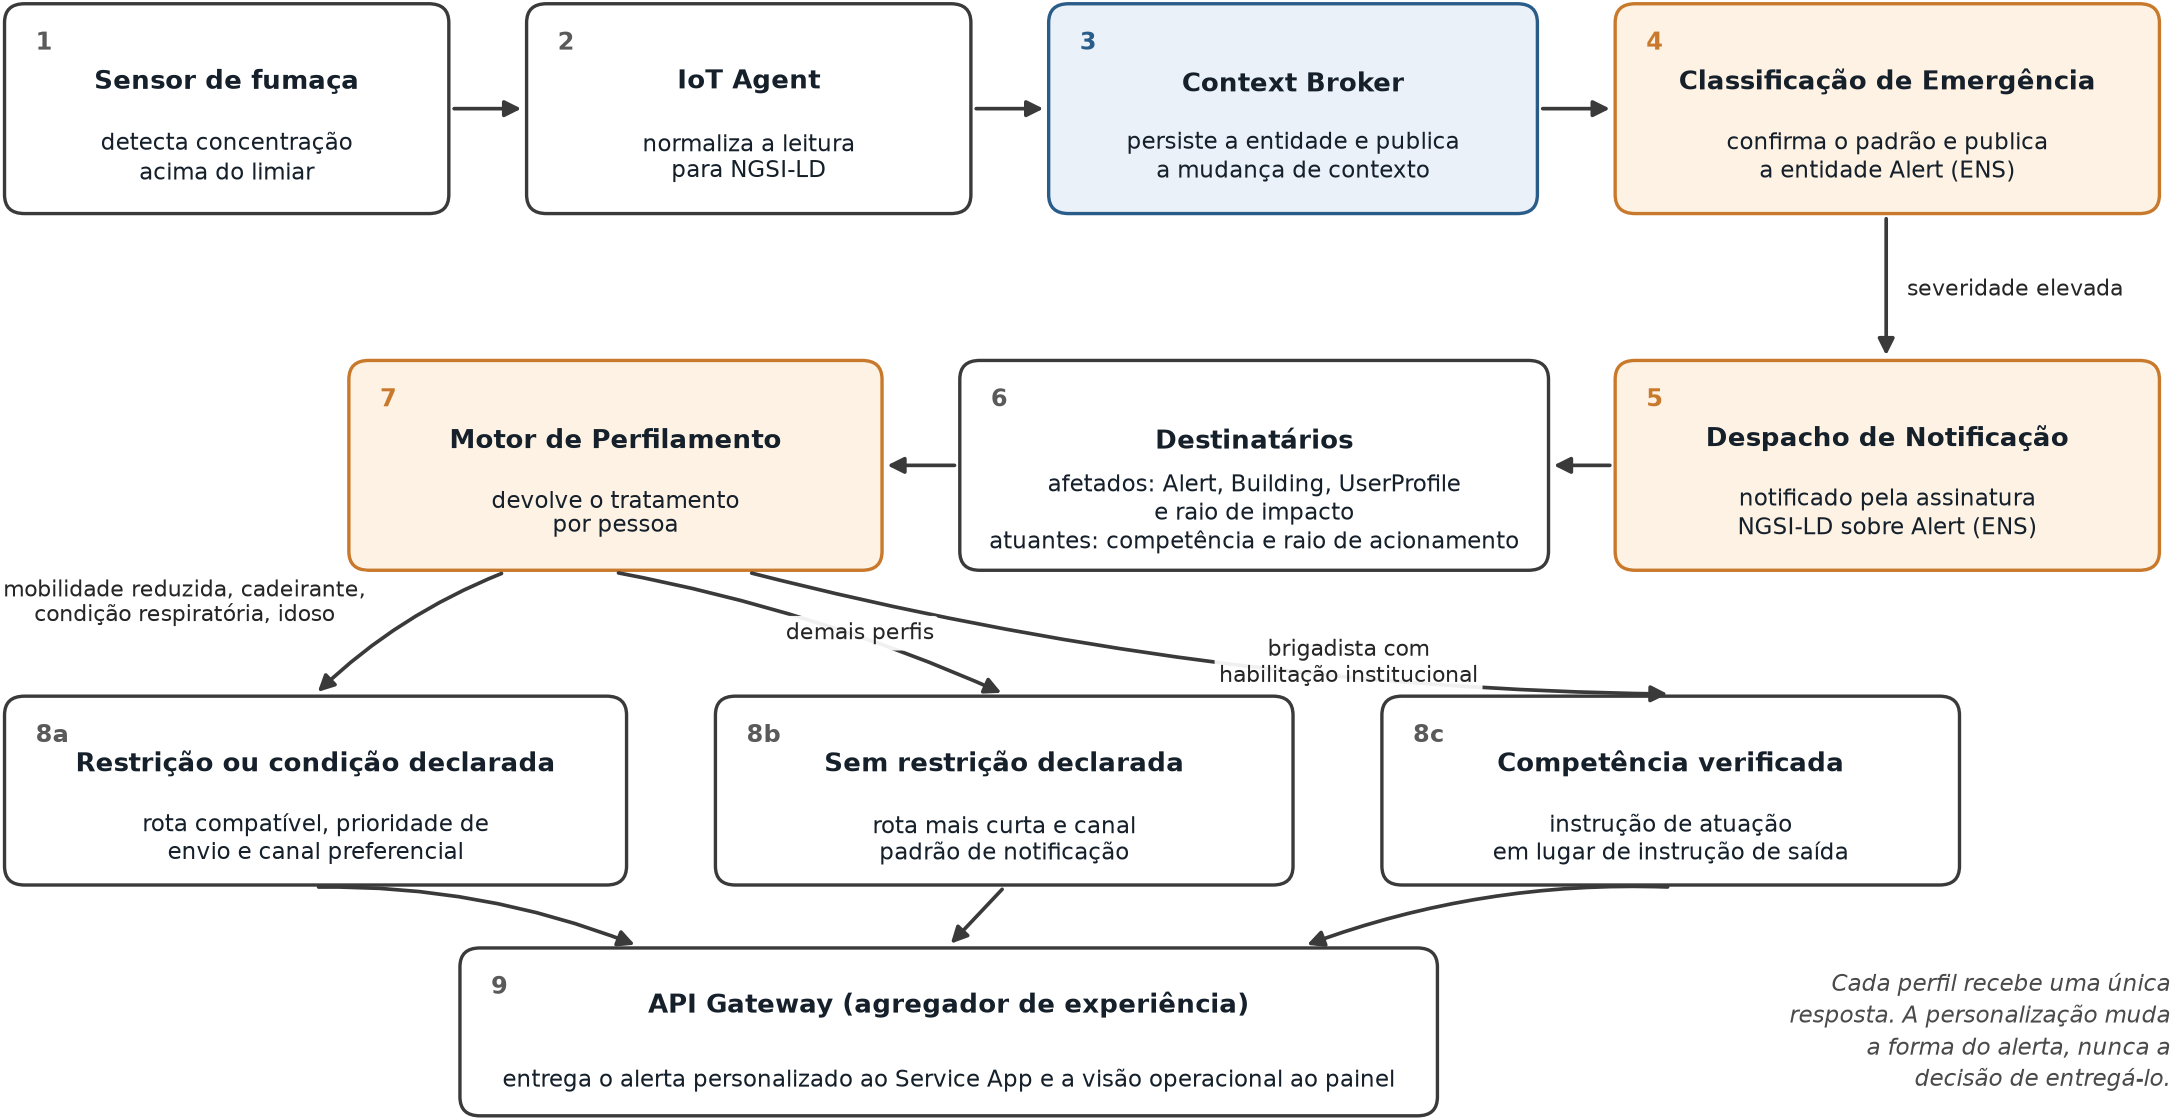
\includegraphics[width=\linewidth]{Imagens/fig_atividades.png}
		\par
		\raggedright
		\footnotesize
		\legend{Fonte: elaborada pelo autor.}
	\end{minipage}
\end{figure}

Um sensor de fumaça em edificação de uso coletivo detecta concentração acima do limiar e reporta a leitura ao agente de dispositivo, que a normaliza para NGSI-LD e a submete ao broker. Validada e persistida a atualização, o \textit{Emergency Classifier} recebe a mudança por assinatura e, confirmado o padrão de incêndio, cria a entidade \texttt{Alert} com severidade elevada e relacionamento \texttt{refersTo} apontando para a edificação.

A criação do alerta satisfaz a assinatura do \textit{Emergency Dispatcher}, que deriva o conjunto afetado combinando a travessia \texttt{Alert}, \texttt{Building}, \texttt{UserProfile} com a consulta geoespacial por raio de impacto, e acrescenta os atuantes pela competência dentro do raio de acionamento. Para cada pessoa do conjunto, o despacho obtém do Motor de Perfilamento o tratamento devido, avaliado contra o escopo de consentimento declarado para a finalidade de resposta a emergência.

As regras são então avaliadas perfil a perfil. Para um cidadão sem restrição declarada, a resposta é o alerta com a rota de saída mais curta pelo canal padrão. Para um cidadão em cadeira de rodas, o cálculo de rota é restrito a segmentos acessíveis e produz itinerário distinto, possivelmente mais longo, porém transitável, e a notificação segue pelo canal sonoro-tátil declarado como preferencial. Para quem declarou condição respiratória ou pertence à faixa etária idosa, o despacho antecipa o envio na fila e a rota prioriza a saída de menor percurso, porque a exposição à fumaça pesa mais nesses casos. \citeonline{deng2022semantic} demonstraram a viabilidade de roteamento sensível às condições do ocupante. O mesmo mecanismo separa também por competência. Um brigadista cuja habilitação tenha sido verificada junto à instituição que a emitiu recebe instrução de atuação em lugar de instrução de saída, esteja ele na edificação ou dentro do raio de acionamento, e o painel de gestão recebe a visão agregada da ocorrência. A diferença importa porque competência que a própria pessoa declara não basta para encarregá-la de resposta a incêndio, e o relacionamento \texttt{providedBy} permite exigir origem institucional nesse caso específico. O mesmo evento urbano produz, portanto, respostas distintas, todas derivadas de atributos que já estão integrados ao grafo da cidade. O \textit{API Gateway} entrega o \textit{payload} à aplicação do cidadão e ao painel de gestão, e a trilha de auditoria registra, por perfil notificado, a regra aplicada e a decisão de autorização que liberou o acesso ao perfil de acessibilidade.
